%% vim: set sts=4 et tw=100 :

\chapter{Library Interface}
\label{ch:interface}

The rationale behind several of the design decisions of the \EOS libraries are
explained in \refsec{interface:design}. We document the core set of \cpp
classes in \refsec{interface:classes}.


\section{Design}
\label{sec:interface:design}

To fulfill its intended use cases, the \EOS libraries are designed by abiding
to the follwing principles.\\

First, scalar quantities are treated as parameters.
These include
\begin{itemize}
    \item experimental inputs, such as particle masses and lifetimes;
    \item theoretically motivated quantities, such as quark masses
        (\eg in the \MSbar scheme) and the Wolfenstein parameters of the CKM matrix.
\end{itemize}
It is therefore straightforward to change a parameter's role from one analysis to the next;
\eg from being a nuisance parameter when producing theory estimates, to being a parameter
of interest when inferring knowedlge from experimental data. To differentiate between the
various parameters, a naming scheme is put in place:
\begin{equation}
    \texttt{NAMESPACE::ID@TAG}\,,
\end{equation}
where the meta variables convey the following meaning:
\begin{description}[leftmargin=!,labelwidth=.15\textwidth]
    \item[\texttt{NAMESPACE}]
            A short description of the context in which the parameter should be
            interpreted. Possible namespaces include, but are not limited to: \texttt{mass},
        \texttt{decay-constants}, \texttt{CKM}, and others. \\
    \item[\texttt{ID}]
            A descriptive handle for the parameter in its namespace.\\
    \item[\texttt{TAG}]
            A forther pices of information that allows to distinguish between
            parameters with the same \texttt{ID}.\\
\end{description}


Second, quantities that exhibit a functional dependence on either a parameter or
a kinematic variable are treated as plugins: An interface is created that
allows implementing more than one realization of the respective function.
The actual implementations of this interface are then accesible
via a factory method.\footnote{%
    A good example for such a modular design is found within the scope of
    hadronic matrix elements, in particular hadronic form factors.
}
Each implementation of a plugin can depend on its own subset of parameters. For
clarity, we use one of the hadronic form factor as an example.
Consider the $B\to \pi$ vector form factor $f^{B\pi}_+$. One possible
parametrization of this form factor has been proposed in \cite{Bourrely:2008za}
(denotes as \option{BCL2008}). It is achieved in terms of three parameters:
\begin{itemize}
    \item the normalization $f^{B\pi}_+(0)$, and
    \item two shape parameters $b^{B\pi,+}_1$ and $b^{B\pi,+}_2$.
\end{itemize}
This parametrization is implemented within \EOS as one of several options for
a $B\to \pi$ form factor parametrization.
The relevant \EOS parameters are contained in the
namespace \texttt{B->pi}, and tagged for the \text{BCL2008} plugin:
\begin{equation}
    \texttt{B->pi::f\_+(0)\@BCL2008}\,,\quad\texttt{B->pi::b\_+\^{}1\@BCL2008}\,,
    \quad\text{and}\quad\texttt{B->pi::b\_+\^{}2\@BCL2008}\,.
\end{equation}
This removes the risk of namespace collisions among the various plugins'
parameters.\\
Observables that depend on the the $B\to \pi$ form factors can be
implemented by relying on the form factors interface, and leave the concrete
parametrization to be a run-time option with name \option{form-factors}.  The
\option{BCL2008} parametrization can be selected by passing
\option{form-factors=BCL2008} to the observable.\\


Third, data is only copied when explicitly requested. Copy constructors yield
another object that points to the same underlying data. This is achieved through
extensive use of the \emph{Private Implementation} design pattern.\footnote{%
    See \url{https://cpppatterns.com/patterns/pimpl.html}.
}
To make an independent copy, the \EOS classes provide the \cpp{clone()} method.


\section{Core Classes}
\label{sec:interface:classes}

At the core of the EOS API there are four classes:
\begin{description}[leftmargin=!,labelwidth=.15\textwidth]
    \item[\class{Parameters}]
        which contains the whole set of \class{Parameter} known to EOS
    \item[\class{Kinematics}]
        which contains the set of kinematic variables specific to one
        instance of \class{Observable}
    \item[\class{Options}]
        which contains the set of options specific to one instance of
        \class{Observable}
    \item[\class{Observable}]
        which encapsulates the numerical implemention of a single
        (pseudo-)observable quantity.
\end{description}

\subsection{Class \class{Parameters}}

Implemented as a dictionary, with keys of type \cpp{std:string} and values of type
\cpp{Parameter}. The default set of parameters is loaded from the \EOS-supplied YAML files. It can be
loaded by using the static \cpp{Parameters::Defaults()} method. Using the copy construtor does not yield
an independent copy; instead the second object uses the underlying data of the initial
instance. To obtain an independent copy with the same values as the present one, use
the \cpp{clone()} method.

\begin{figure}[t]
    \centering
    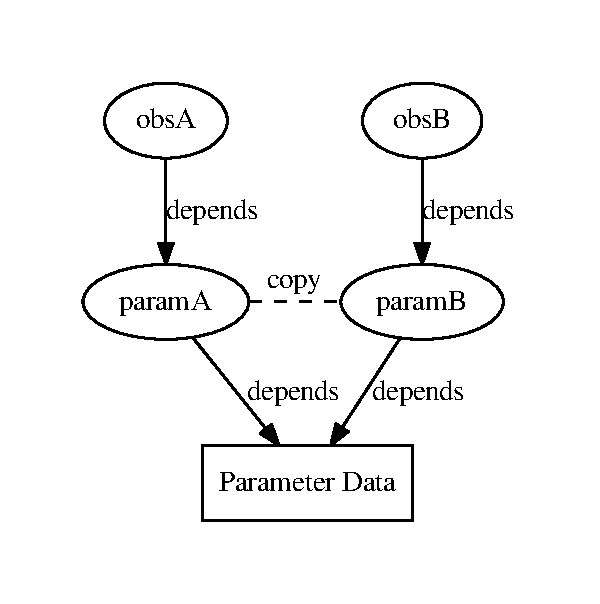
\includegraphics[width=.5\textwidth]{figures/graph-parameters.pdf}
    \caption{%
        Diagrammatic illustration that multiple observables can depend on the
        very same instance of \cpp{Parameters}.
    }
\end{figure}

\begin{sourcecode}
Parameters paramA = Parameters::Defaults();
Parameters paramB(paramA);

ObservablePtr obsA = Observable::make("A", paramA, Kinematics{ }, Options{ });
ObservablePtr obsB = Observable::make("A", paramB, Kinematics{ }, Options{ });
\end{sourcecode}

You can access individual parameters via the array subscript operator. It takes
a \cpp{class QualifiedName} object as its key, which can be created implicitly
from \cpp{std::string} or \cpp{const char *}. You can also iterate over all
parameters via the \cpp{begin()} and \cpp{end()} methods. In both cases, the
underlying objects are of \cpp{class Parameter}, which provides access to
the current value via the \cpp{evaluate()} method.


\subsection{Class \class{Kinematics}}

The class \class{Kinematics} is a dictionary from \cpp{std::string}-valued keys to
\cpp{KinematicVariable}-valued entries. Upon construction of an observable, a suitable instance
of kinematics is bound to that observable. Acces to individual kinematic variables
occurs through the array subscript operator.
The class is used for the run-time construction of observables. For this purpose,
the variable names apply only to a single observable and are not explicitly namespaced.


\subsection{Class \class{Options}}

The class \class{Options} is a dictionary from \cpp{std::string}-valued keys to
\cpp{std::string}-valued entries. Upon construction of an observable, a suitable instance
of \class{Options} is bound to that observable. The underlying class's constructor
queries the options, and select the appropriate run-time behaviour.\\

Helper classes are available for repeated options-related task, \eg the class
\class{SwitchOption}.


\subsection{Class \class{Observable}}

The class \class{Observable} is an abstract base class. To create a new observable object,
you must use the static \class{Observable::make()} factory method. It requires three arguments:
\begin{itemize}
    \item a \cpp{class QualifiedName} object \cpp{n};
    \item a \cpp{class Parameters} object \cpp{p}; and
    \item a \cpp{class Kinematics} object \cpp{k}; and
    \item an \cpp{class Options} object \cpp{o}.
\end{itemize}

To allow for more compact code, \EOS' internal observables are not implemented as individual
classes. Instead, related observables are bundled together into one class. Individual observable
classes are then created using the \cpp{template <...> class ConcreteObservable}. We refer to
\refsec{extending:observable} for details on how to extend \EOS with the implementation
of a new observable.\\


\emph{Note}: Any changes to the \class{Options} object \cpp{o} after construction of the observable
do not affect the observable.\\


\emph{Note}: All users of \class{Observable} must also support cloning. This allows to easily
parallelize algorithms acting on \class{Observable}.

\begin{figure}
    \subfigure[copy]{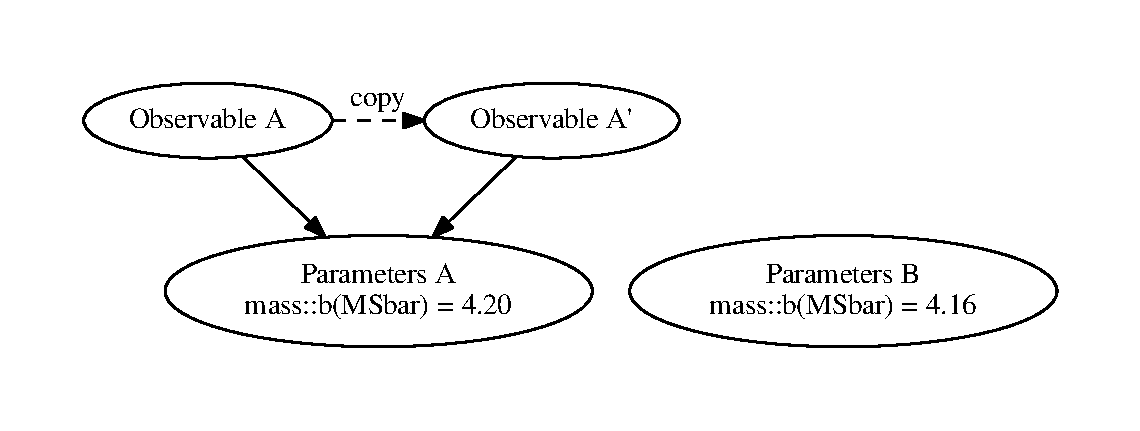
\includegraphics[width=.5\textwidth]{figures/graph-observable-copy.pdf}}
    \subfigure[clone]{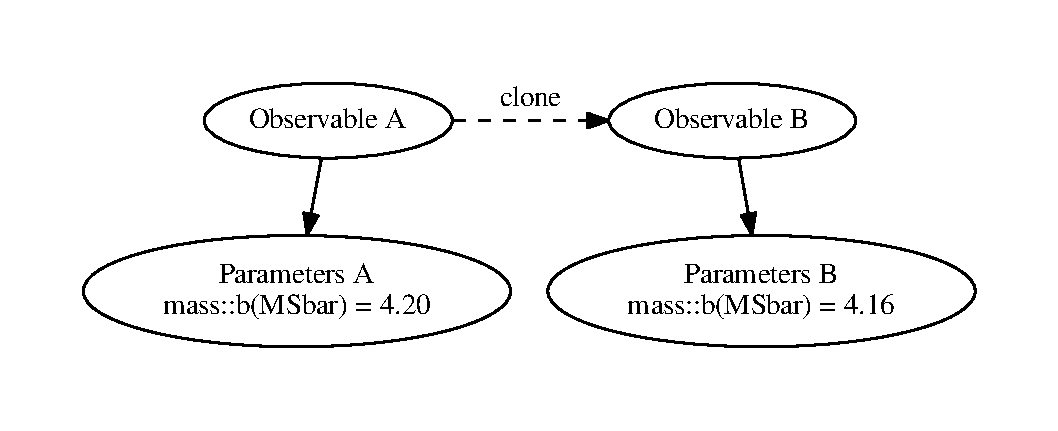
\includegraphics[width=.5\textwidth]{figures/graph-observable-clone.pdf}}
    \caption{%
        Diagrammatic illustration of the differences between copying an instance of
        \cpp{Observable} via the copy-constructor, and cloning the observable via the \cpp{clone}
        method
    }
\end{figure}
